%!TEX root = ../3dchapter.tex

\setchapterpreamble[u]{\margintoc}

\graphicspath{{gmaps/}}
\renewcommand*{\thelesson}{4.2}

\chapter{Generalised and combinatorial maps}%
\label{chap:gmaps}

Generalised maps and combinatorial maps are two related data structures to represent objects of any dimension using a single consistent definition.
2D combinatorial maps are basically the same as most half-edge data structures, with the minor difference that the links between primitives are defined in a manner that works consistently in every dimension.
However, they have clear advantages when we move to 3D combinatorial maps, in which we can break the limits of boundary representation and can store links between adjacent volumes.

As for generalised maps, they are very similar to the combinatorial maps of the same dimension, but they avoid the concept of orientation at the cost of having twice as many primitives.
Theoreticians thus mostly focus on how generalised maps can represent unorientable objects.
However, the most interesting aspect about them is that by omitting orientation, they make building many algorithms easier.

Higher-dimensional generalised and combinatorial maps (\ie\ 4D and higher) can be used to incorporate other non-spatial features, such as time and scale, although this is more of a research topic than a practical application.

\section{What are generalised and combinatorial maps?}

\emph{Generalised maps} (\emph{g-maps}) and \emph{combinatorial maps} (\emph{c-maps} or just \emph{maps}) are what are known as \emph{ordered topological models}.
These are subdivisions of space into abstract simplices (Figure~\ref{fig:simplices}), much like a geometric triangulation in 2D or a tetrahedralisation in 3D.
However, unlike the latter, the subdivision operation to create an ordered topological model is a purely combinatorial operation, \ie\ no geometric tests are ever made.

\begin{figure}
\centering
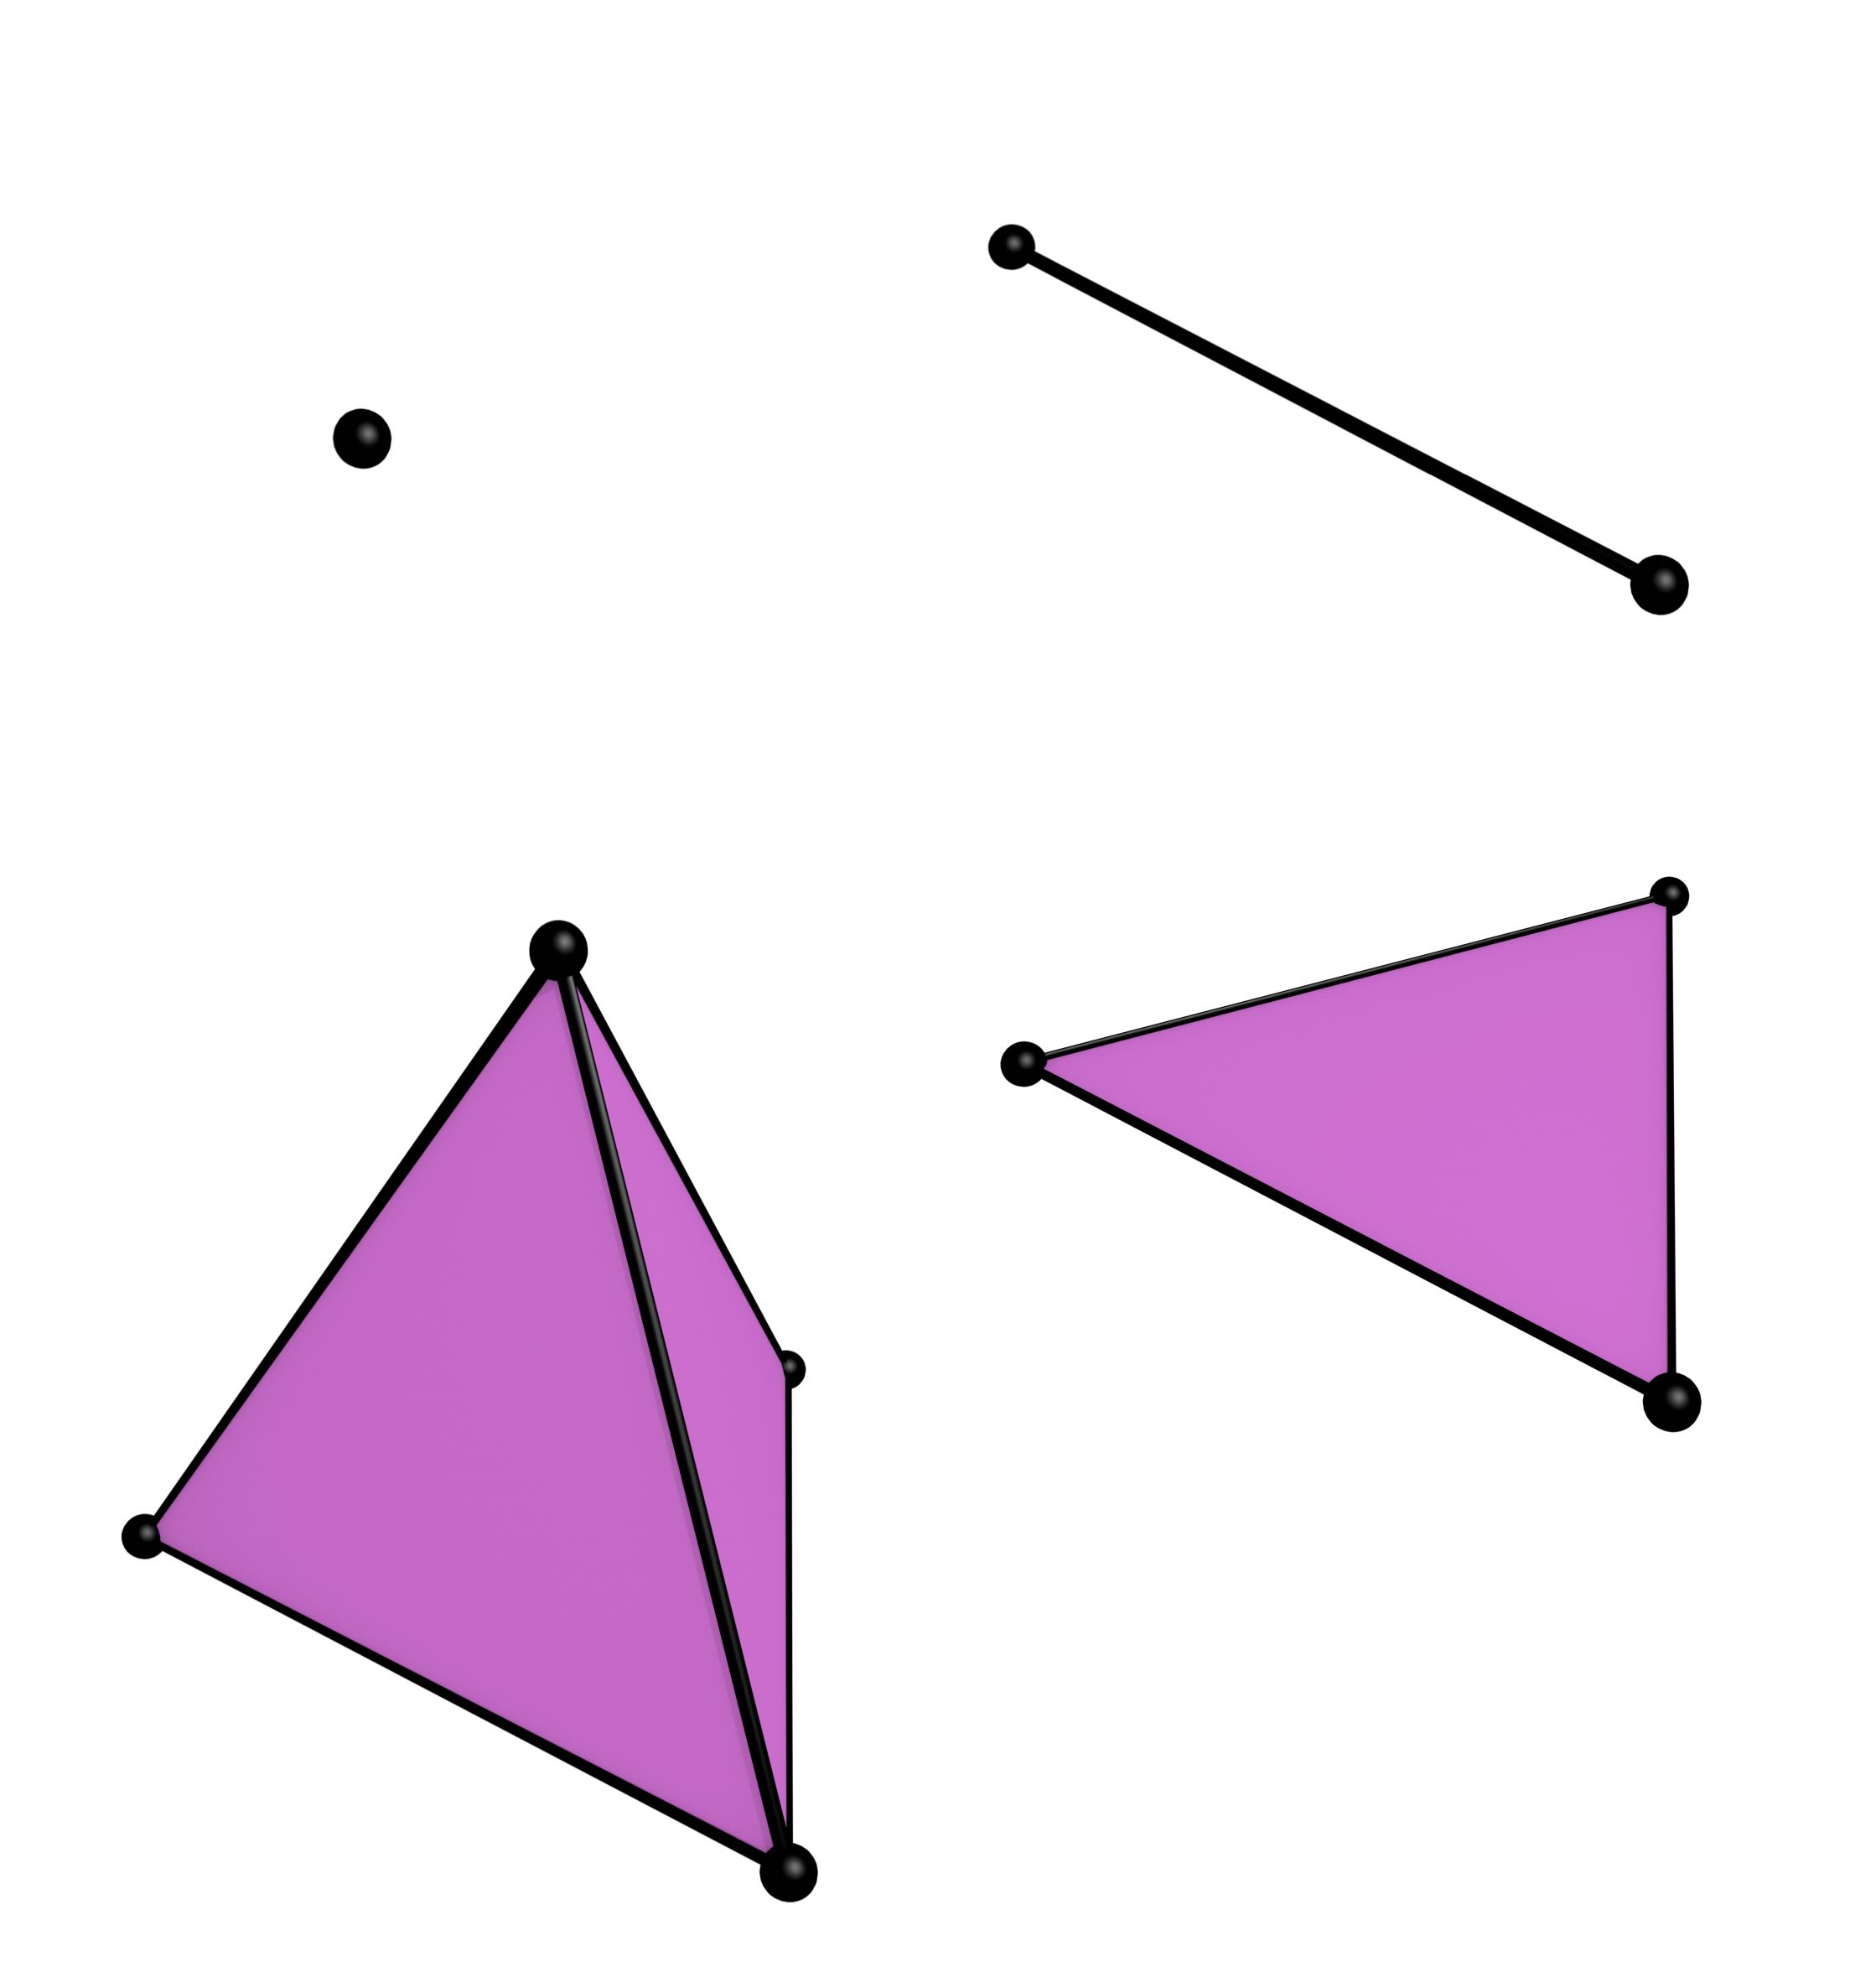
\includegraphics[width=0.5\linewidth]{figs/simplex}
\caption{An \(n\)-dimensional simplex, or simply \(n\)-simplex, is a combinatorial primitive made from a set of \(n+1\) vertices.
A 0-simplex is thus a point, a 1-simplex is a line segment, a 2-simplex is a triangle, and a 3-simplex is a tetrahedron.
Here they are shown as if embedded in 3D space (\ie\ \(\mathbb{R}^3\)).}%
\label{fig:simplices}
\end{figure}

At this point, it is very important to note that the simplices in an ordered topological model \emph{do not correspond to actual simplices in space}, \ie\ they do not represent actual triangles or tetrahedra that you can point to in a 3D model.
However, there are a few geometric interpretations that are possible, and we will be using one of them to help in understanding, but please bear in mind that it is slightly incorrect from a theoretical standpoint.

\subsection{Darts}

The most precise geometric interpretation is as follows: a generalised or combinatorial map is akin to a barycentric triangulation.
Shortly, a barycentric triangulation of a polygon is a simple way to triangulate a roughly convex polygon by adding a new vertex at its barycentre, then creating new triangles by joining this new vertex to every existing edge in the triangulation, \ie\ forming new triangles with the two vertices on the ends of every existing edge plus the new vertex at the barycentre.
This method creates more triangles than are absolutely necessary in a triangulation, but it does so without doing any geometric tests (unlike a constrained triangulation).

In a 2D combinatorial map, the triangulation that is performed is similar to what was described above (Figure~\ref{subfig:cmaps-simplices}), with the difference that the new vertex is not really located at the barycentre.
In fact, that vertex is not located anywhere---hence why the simplices created using this process are called \emph{abstract simplices}.
In the figures, we thus place the new vertex in a convenient location that avoids visually overlapping simplices, but this is just an arbitrary choice to make the figures clearer.

In a 2D generalised map, the barycentric triangulation requires an extra step where we first split every edge into two by adding a vertex at their barycentres (which is equivalent to a barycentric 1D triangulation of the edge), and then do the 2D triangulation as described above (Figure~\ref{subfig:gmaps-simplices}).
Note that this means that a generalised map has exactly twice as many simplices as a combinatorial map of the same model.

\begin{figure}
\centering
\begin{subfigure}{0.3\linewidth}
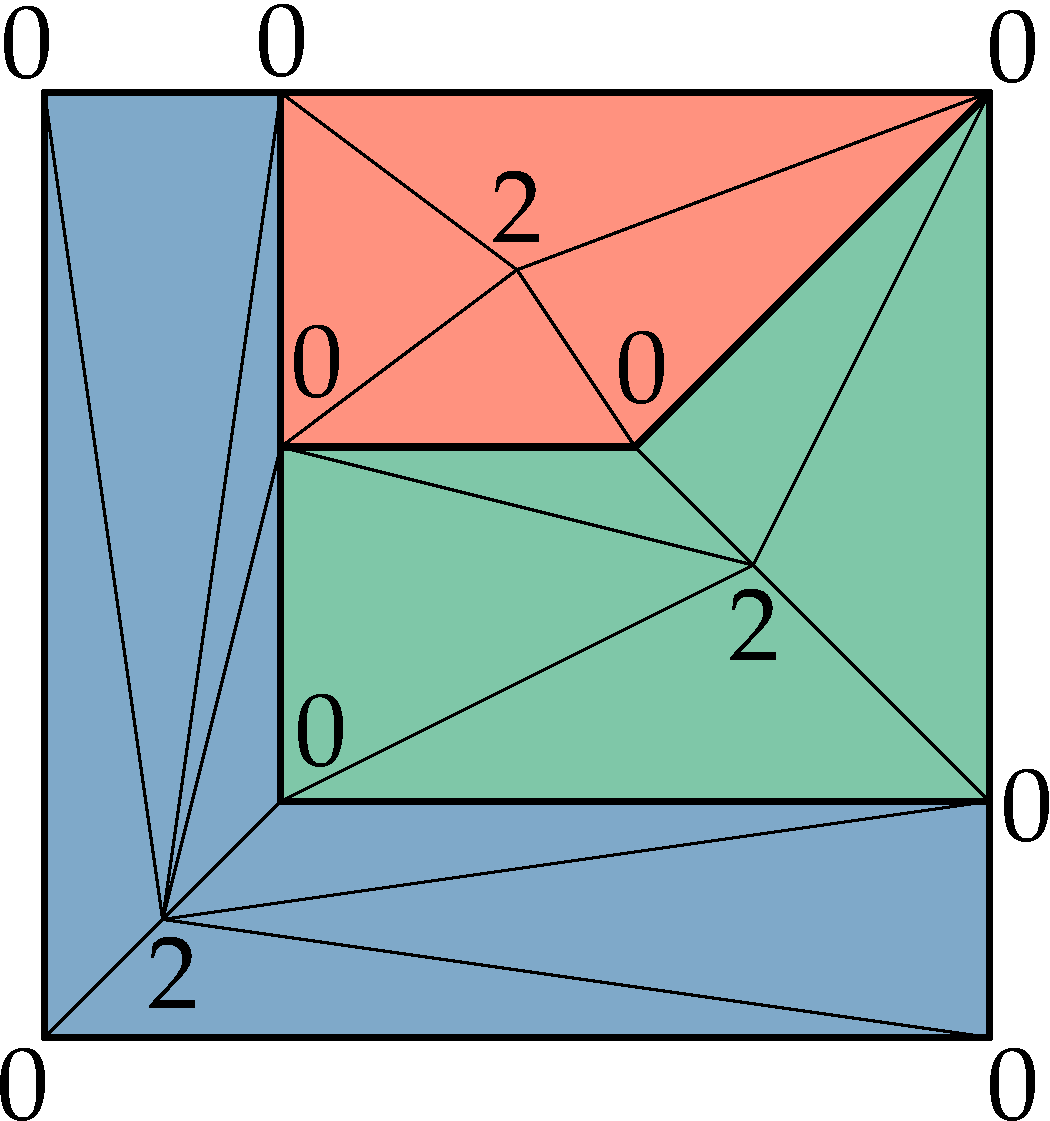
\includegraphics[width=\linewidth]{figs/cmaps-simplices}
\caption{}%
\label{subfig:cmaps-simplices}
\end{subfigure}
\quad
\begin{subfigure}{0.3\linewidth}
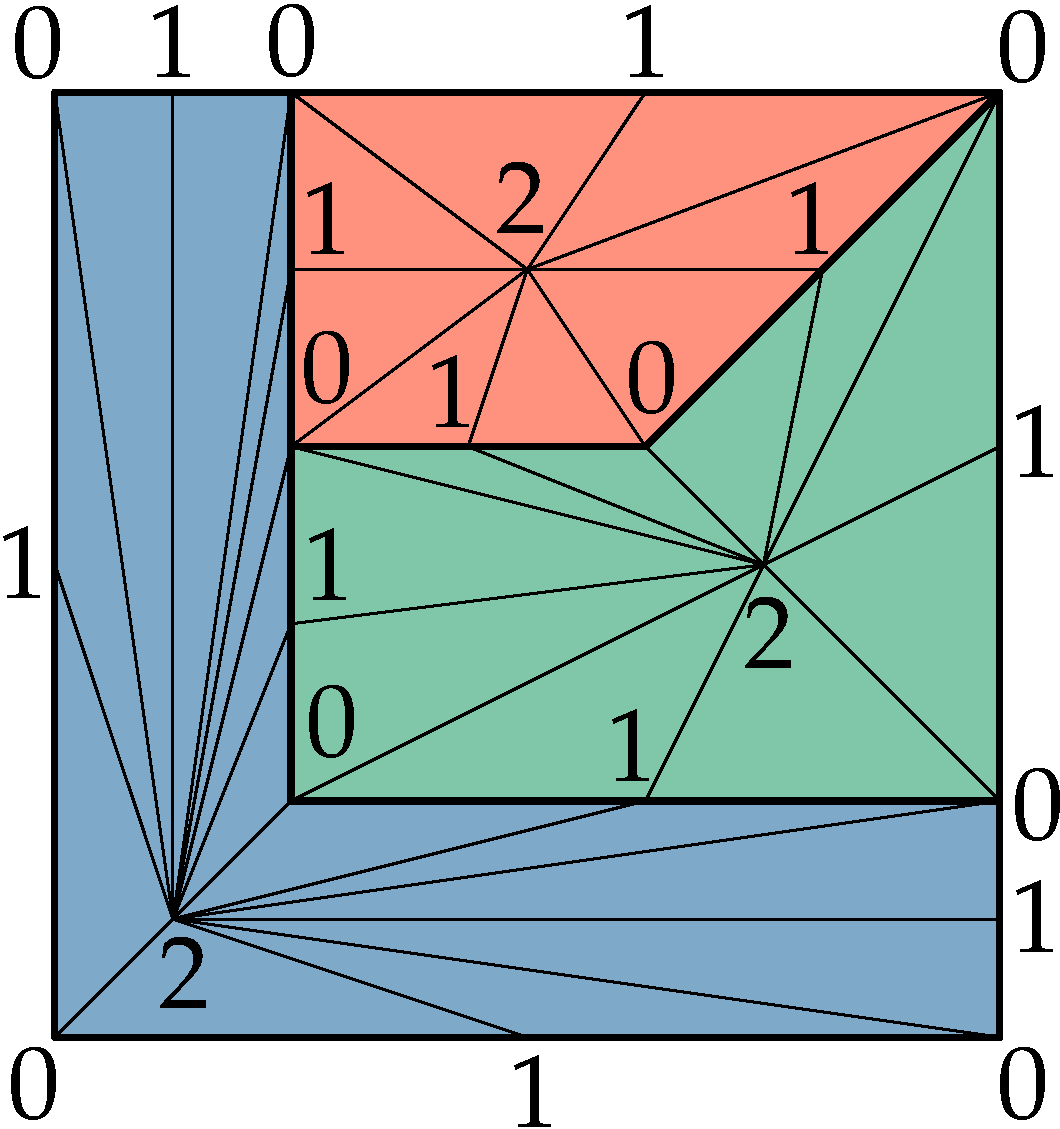
\includegraphics[width=\linewidth]{figs/gmaps-simplices}
\caption{}%
\label{subfig:gmaps-simplices}
\end{subfigure}\\
\caption{The barycentric triangulation interpretation of: (a) a 2D combinatorial map and (b) a 2D generalised map}%
\label{fig:maps-simplices}
\end{figure}

Now, this is where the \emph{ordered} part of an ordered topological model comes in.
Every vertex in the simplices that were created can be associated with an element of a certain dimension.
The original vertices are zero-dimensional, the new vertices on the edges (for g-maps) are one-dimensional, the new vertices on the faces are two-dimensional, and so on.
Doing so reveals that:

\begin{itemize}
\item every simplex in a 2D generalised map has one vertex of every dimension (\ie\ \(0\), \(1\) and \(2\)), and
\item every simplex in a 2D combinatorial map has two zero-dimensional vertices and one two-di\-men\-sio\-nal vertex (\ie\ \(0\), \(0\) and \(2\)).
\end{itemize}

In order to get the tetrahedralisation for a 3D generalised or combinatorial map, we start from the triangulation describing the 2D generalised or combinatorial map of every face, and then we tetrahedralise by adding a new vertex in the barycentre of each volume.
This new vertex is connected to every existing triangle to form the new tetrahedra, which follow the same ordering pattern as before (Figure~\ref{fig:cmap-3d}).
Formulating it in a dimension-independent way, we have that:

\begin{figure}
\centering
\begin{subfigure}{0.33\linewidth}
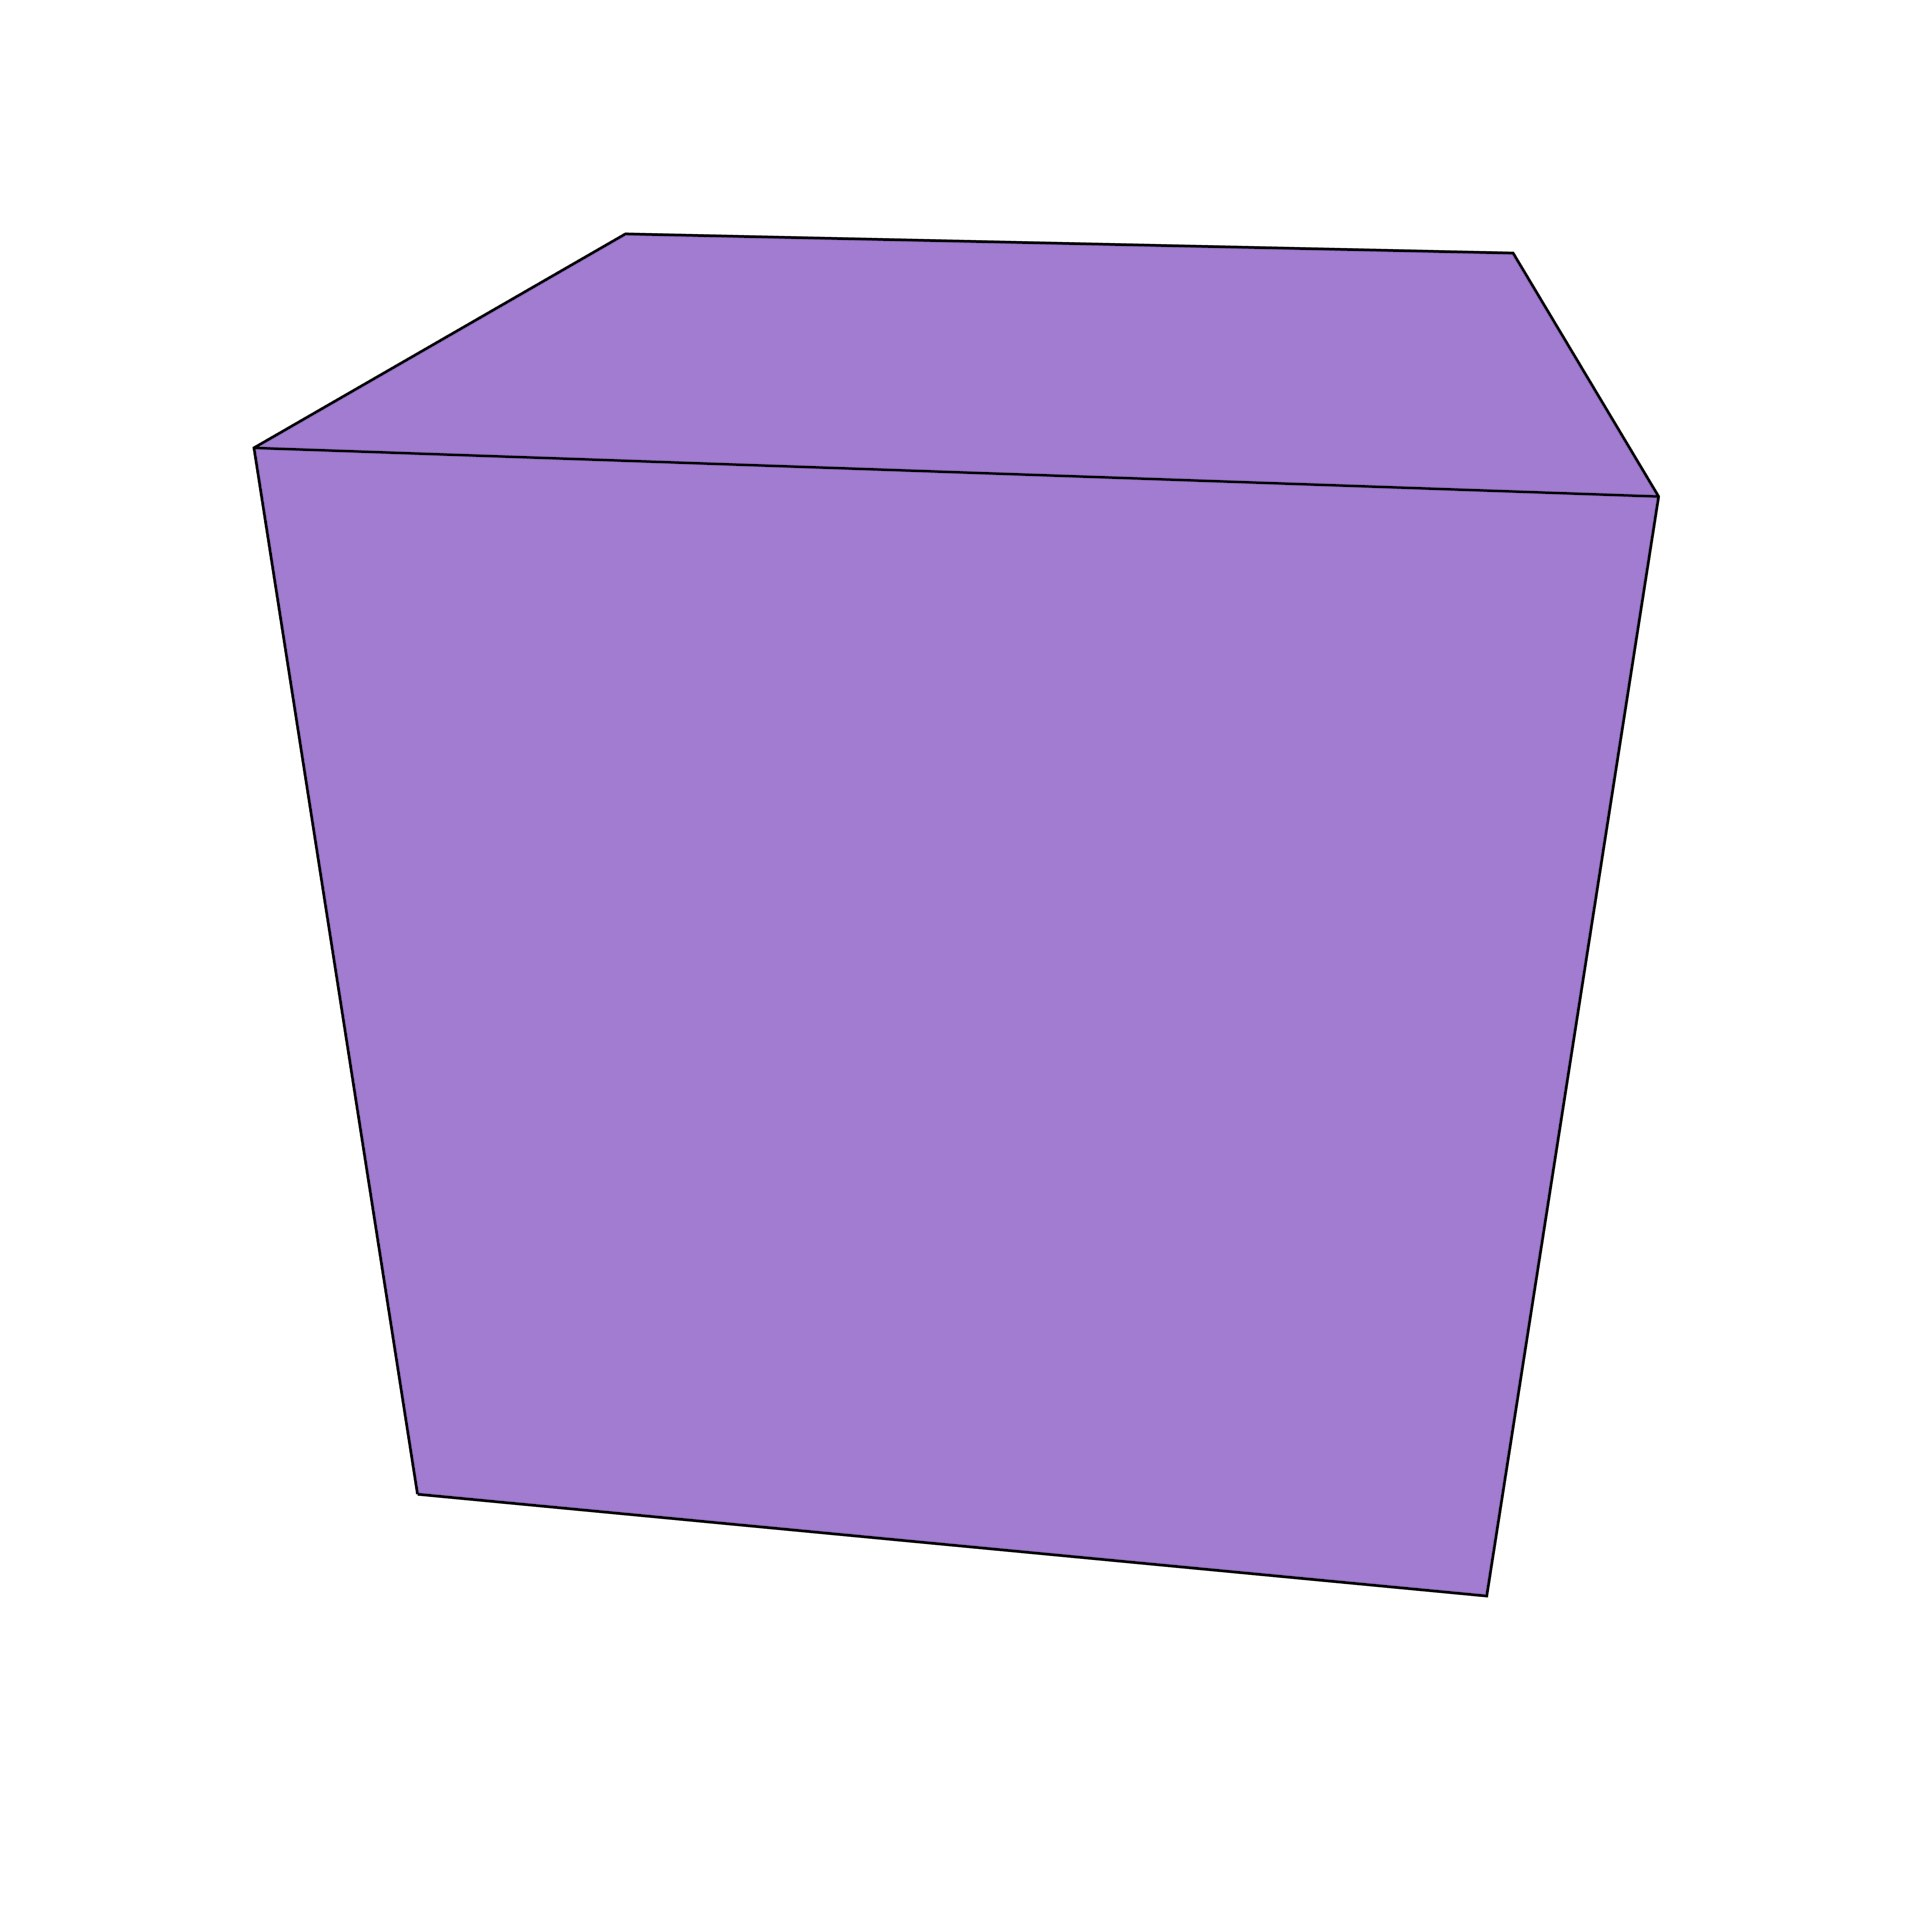
\includegraphics[width=\linewidth]{figs/cube}
\caption{}%
\label{subfig:cube}
\end{subfigure}%
\begin{subfigure}{0.33\linewidth}
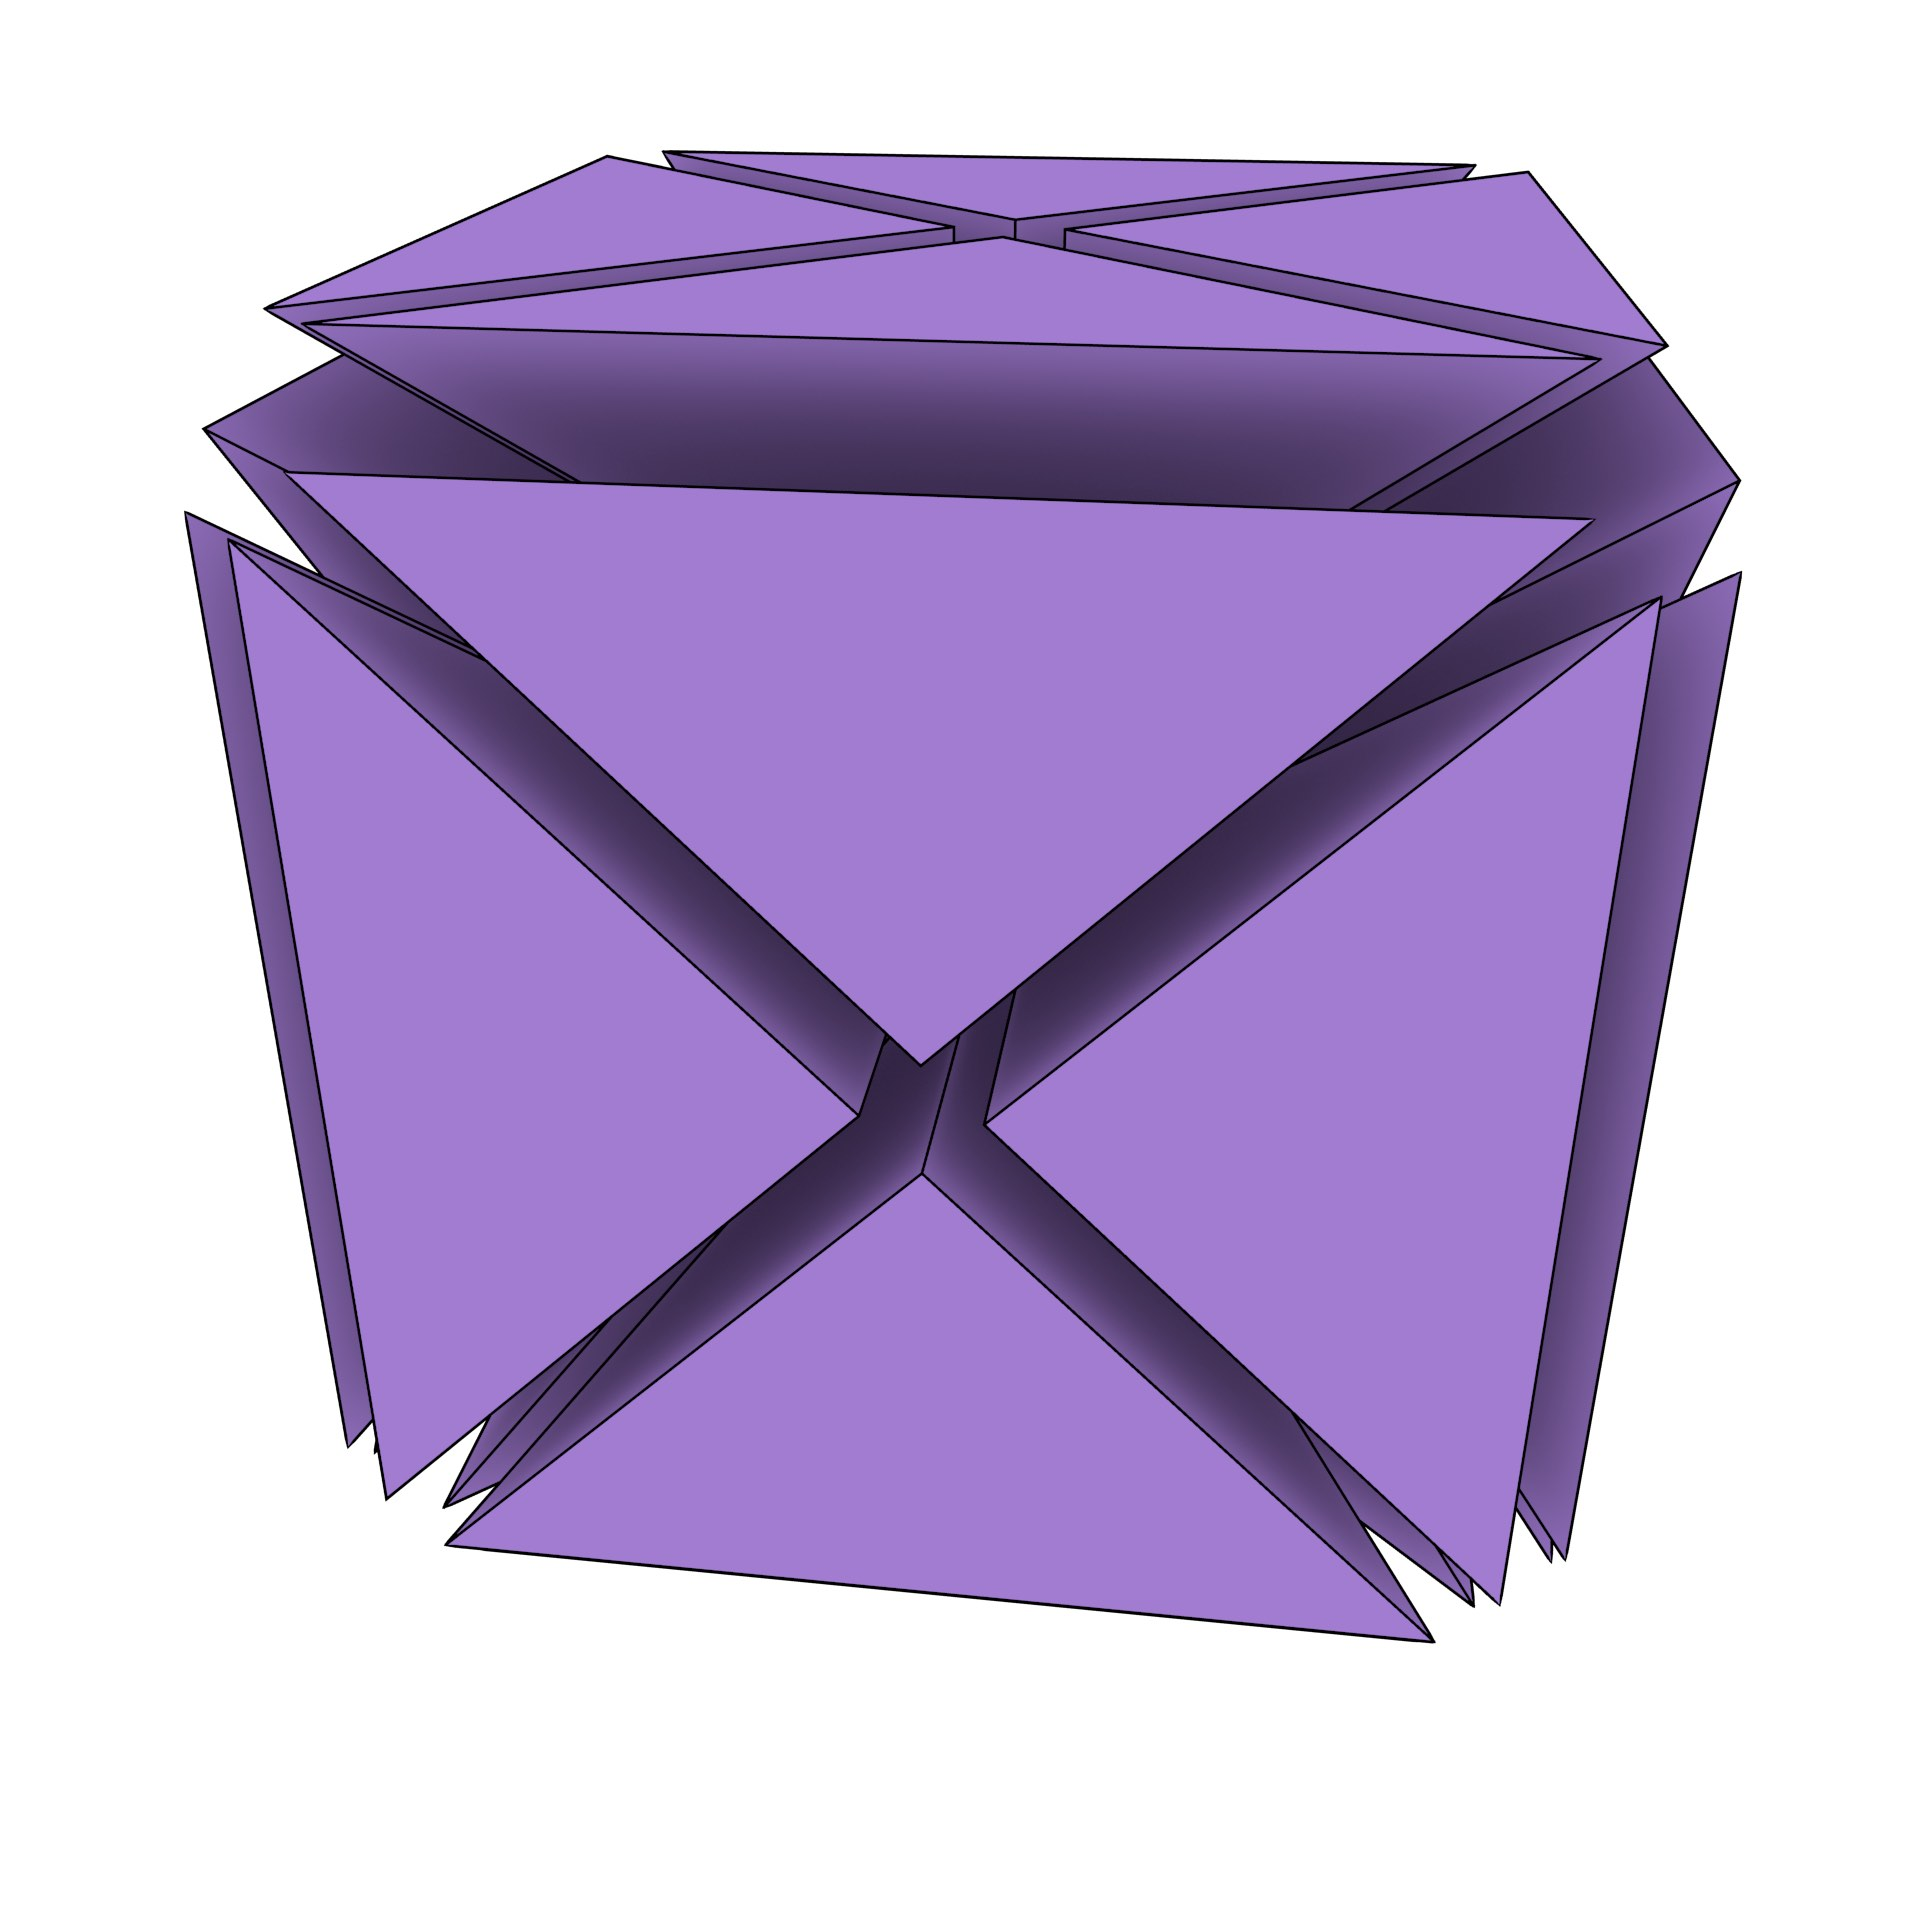
\includegraphics[width=\linewidth]{figs/cmap-3d}
\caption{}%
\label{subfig:cmap-3d}
\end{subfigure}%
\begin{subfigure}{0.33\linewidth}
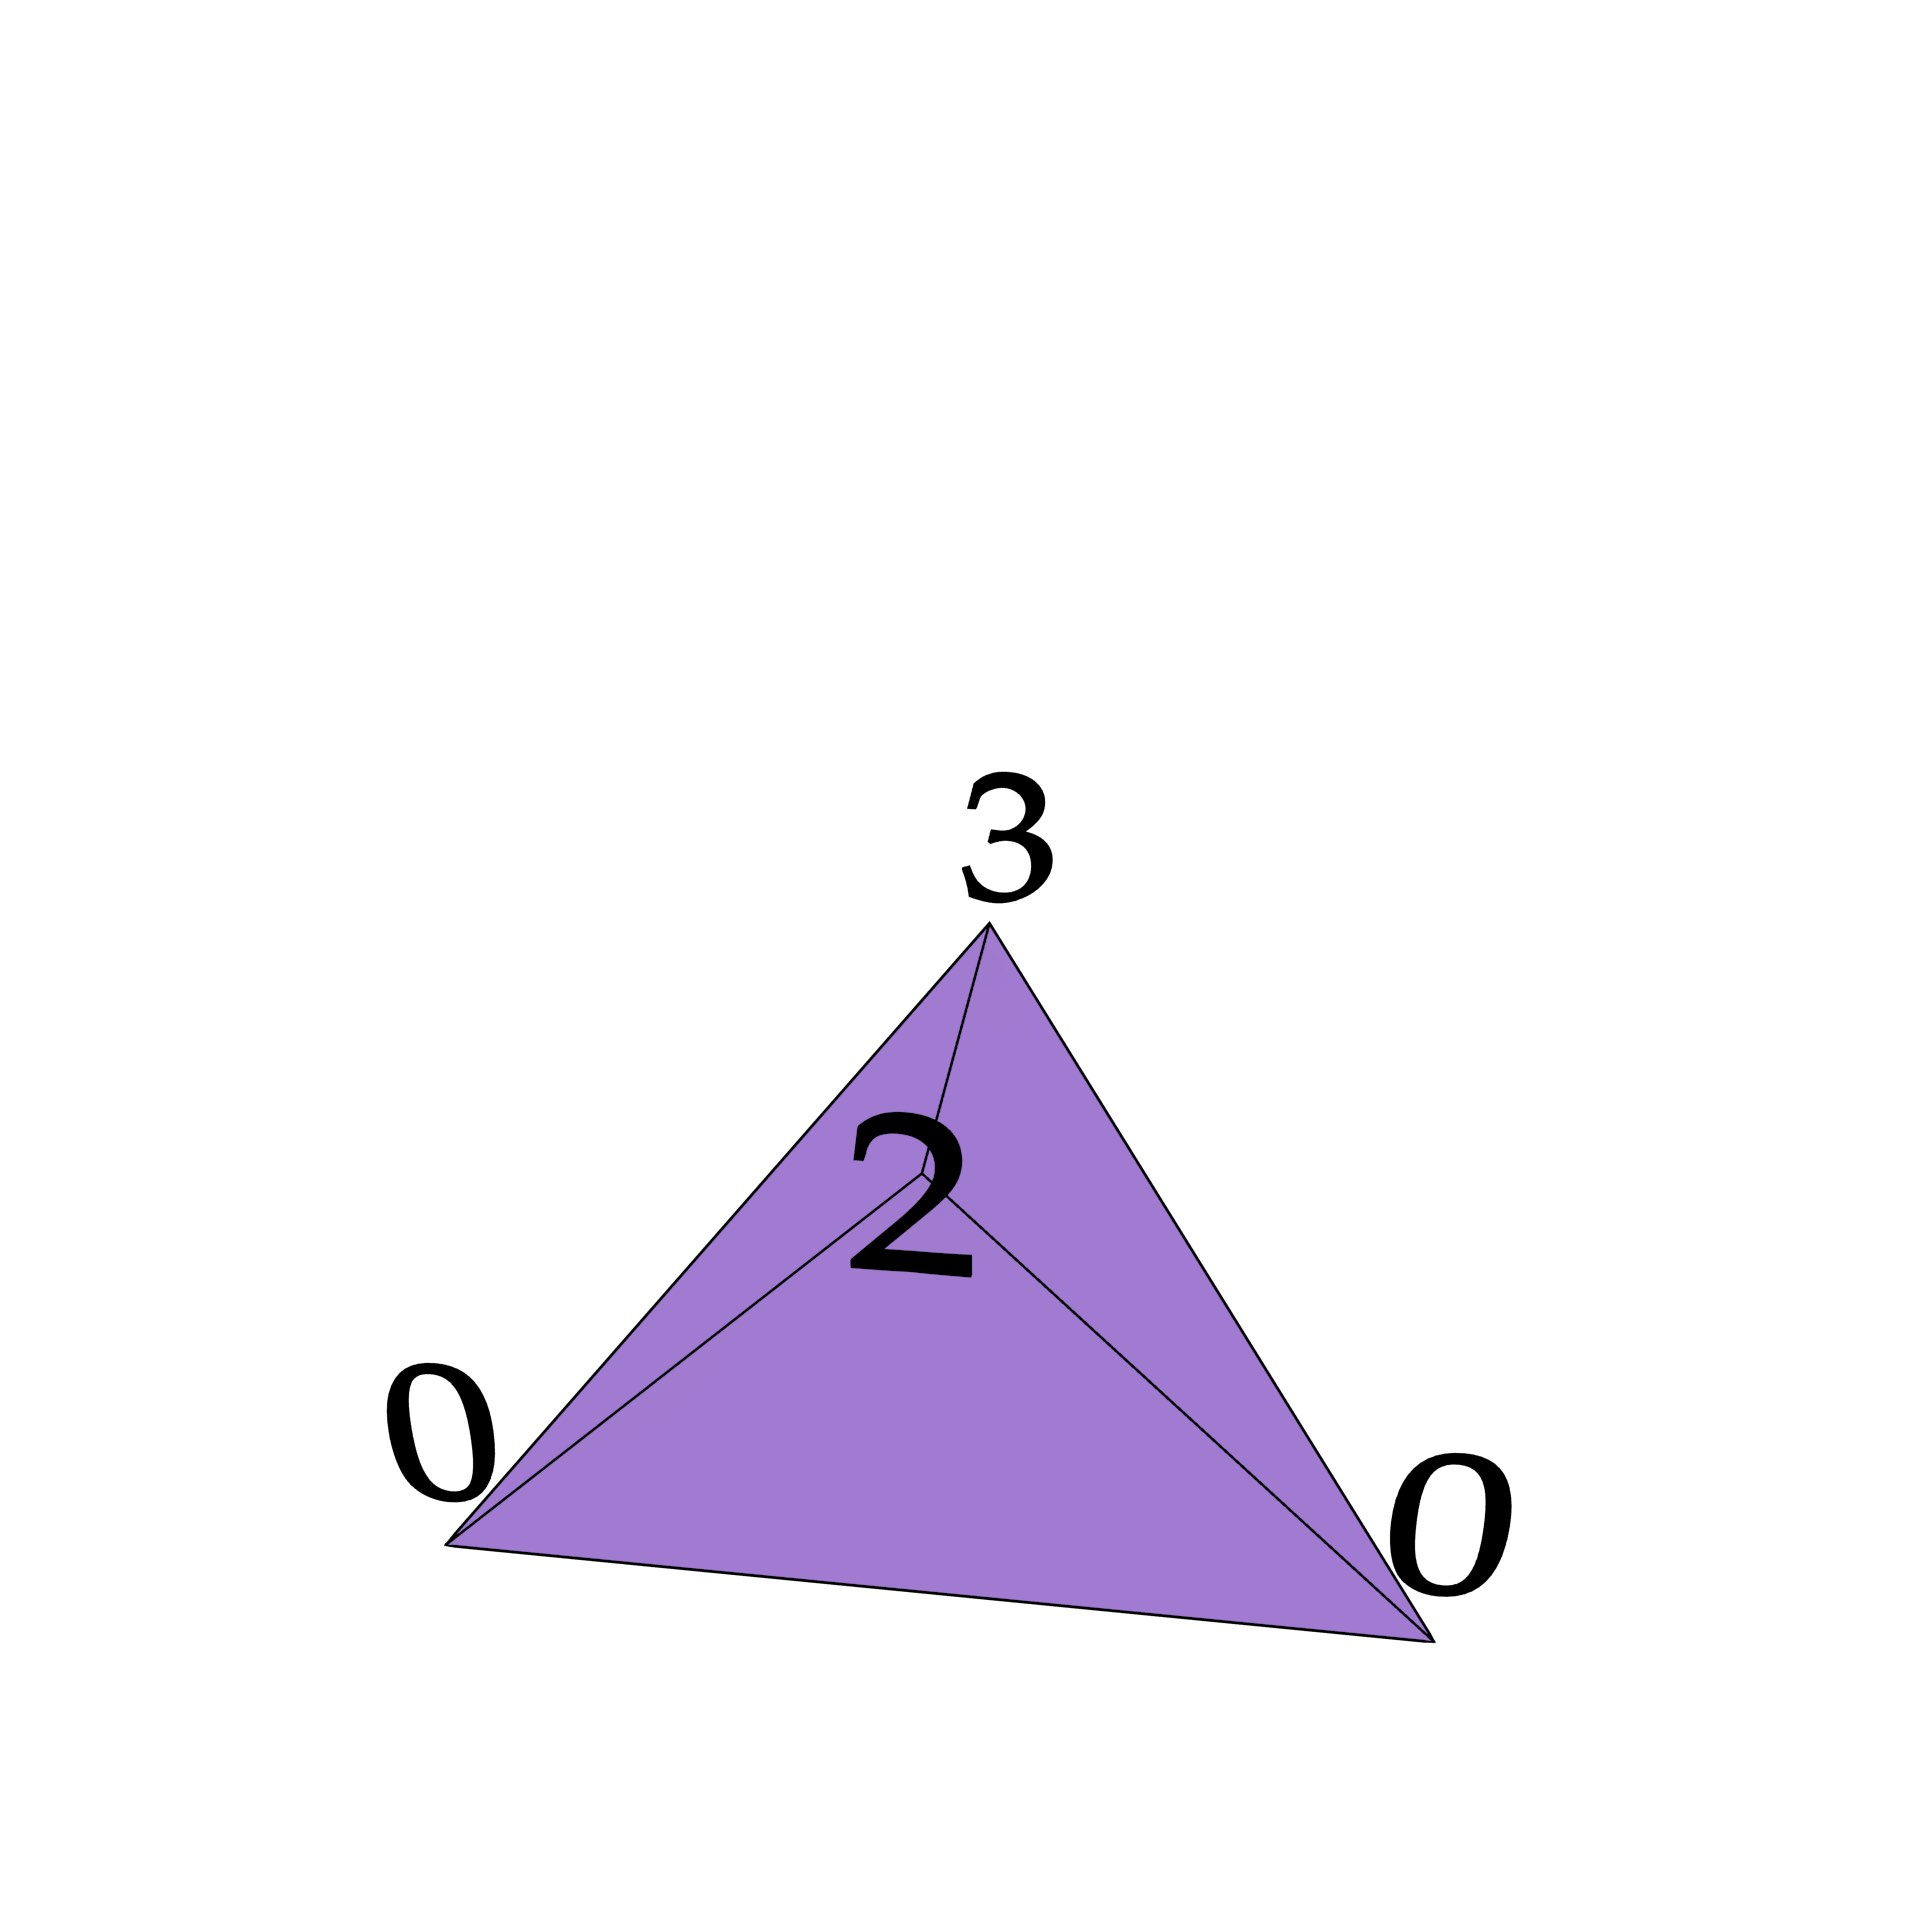
\includegraphics[width=\linewidth]{figs/cmap-3d-vertices}
\caption{}%
\label{subfig:cmap-3d-vertices}
\end{subfigure}\\
\caption{(a) A cube, (b) its barycentric tetrahedralisation for a 3D combinatorial map, and (c) one of its simplices showing the ordered property.}%
\label{fig:cmap-3d}
\end{figure}

\begin{itemize}
\item every simplex in an \(n\)D generalised map has one vertex of every dimension up to \(n\) (\ie\ \(0, 1, 2, \ldots, n\)), and
\item every simplex in an \(n\)D combinatorial map has two zero-dimensional vertices and one one vertex of every dimension from \(2\) up to \(n\) (\ie\ \(0, 0, 2, \ldots, n\)).
\end{itemize}

In a generalised or combinatorial map, the primitives that are used to describe the geometry of objects are precisely these \(n\)D abstract simplices, which are called \emph{darts}.

\subsection{Permutations and involutions}

Let us define some properties of \(n\)-simplices that are important for generalised and combinatorial maps.
An \(n\)-simplex can have up to \(n+1\) adjacent other simplices as neighbours, where adjacency is defined as sharing a common \((n-1)\)-simplex on its boundary.
That is, a line segment can have up to two adjacent line segments (each sharing a vertex), a triangle can have up to three adjacent triangles (each sharing an edge), a tetrahedron can have up to four adjacent tetrahedra (each sharing a triangular face), and so on.
Note that these numbers will be lower for the simplices on the boundary of the model.

Therefore, a dart in a 2D generalised/combinatorial map will have up to three neighbouring darts, whereas a dart in a 3D generalised/combinatorial map will have up to four neighbouring darts, and these neighbours will have all but one of the same vertices as the original dart.
Since two adjacent \(n\)-simplices will have a common \((n-1)\)-simplex on their common boundary, going from a dart to its adjacent neighbour will therefore switch only one of its vertices.
Then, since the ordered property tells us the exact combination of dimensional elements that any simplex must have, the switch must exchange an element of a certain dimension for another element of the same dimension (while keeping all of the other previous elements).

In a generalised map, the operation to change the \(0\)-dimensional element, known as \(\alpha_0\), will thus switch a vertex for another vertex on the same edge, face and volume.
Similarly, the operation to change the \(1\)-dimensional element (\(\alpha_1\)) will switch an edge for another edge on the same vertex, face and volume, the operation to change the \(2\)-dimensional element (\(\alpha_2\)) will switch a face for another face on the same vertex, edge and volume, and the operation to change the \(3\)-dimensional element (\(\alpha_3\)) will switch a volume for another volume on the same vertex, edge and face.
These are thus all denoted as \(\alpha_i\), where \(i\) is the dimension of the element being switched.

In a combinatorial map, the operations are slightly different because of the two \(0\)-dimensional elements, which means that changing either \(0\)-dimensional element will switch an \emph{edge} for either of its two adjacent edges.
Since having an operation that yields two different results is undesirable, we therefore have to choose one of these edges as a result of the operation, which means giving the combinatorial map an \emph{orientation} (Figure~\ref{fig:cmaps-orientation}).
This orientation is defined by ordering the two \(0\)-dimensional elements in the dart, and as in half-edge data structures, two darts connected by an involution should have \emph{opposite orientations}.
Since this operation switches the edges of a dart, it is thus denoted as \(\beta_1\).
As for the other operations, they are defined as in a generalised map, but they are all denoted as \(\beta_i\), where \(i\) is the dimension of the element being switched.

\begin{figure}
\centering
\begin{subfigure}{0.33\linewidth}
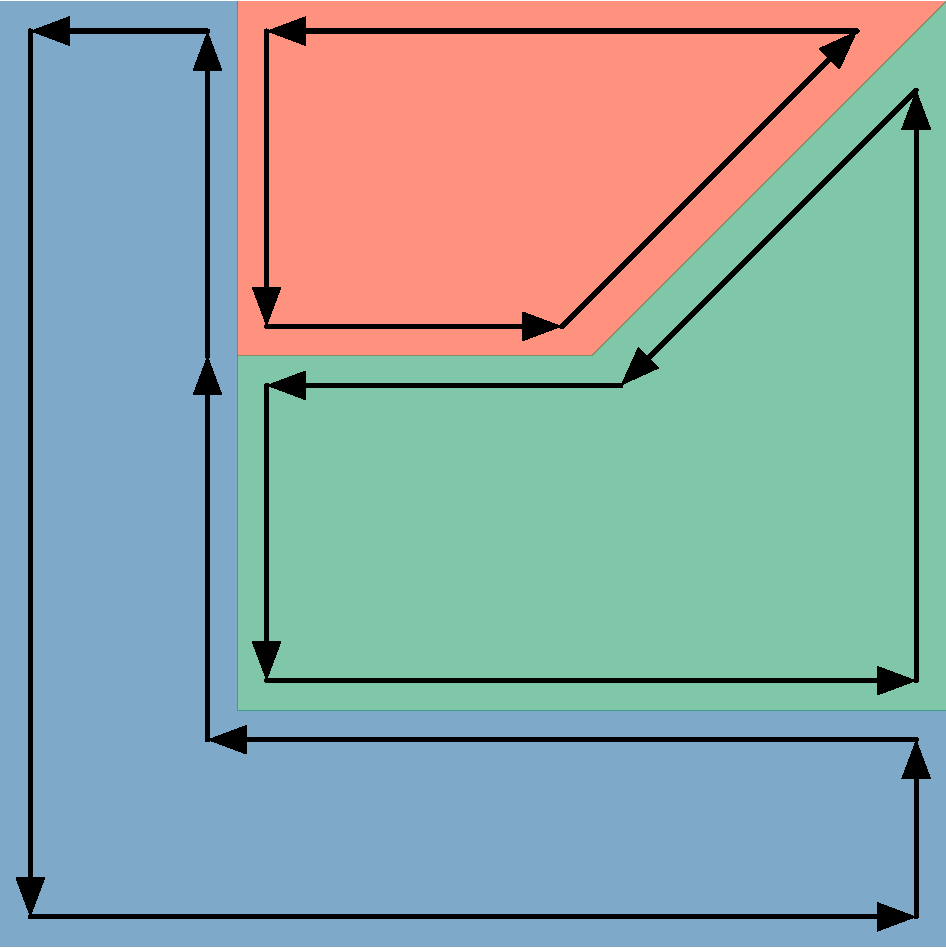
\includegraphics[width=\linewidth]{figs/cmaps-orientation-1}
\caption{}%
\label{subfig:cmaps-orientation-1}
\end{subfigure}%
\quad
\begin{subfigure}{0.33\linewidth}
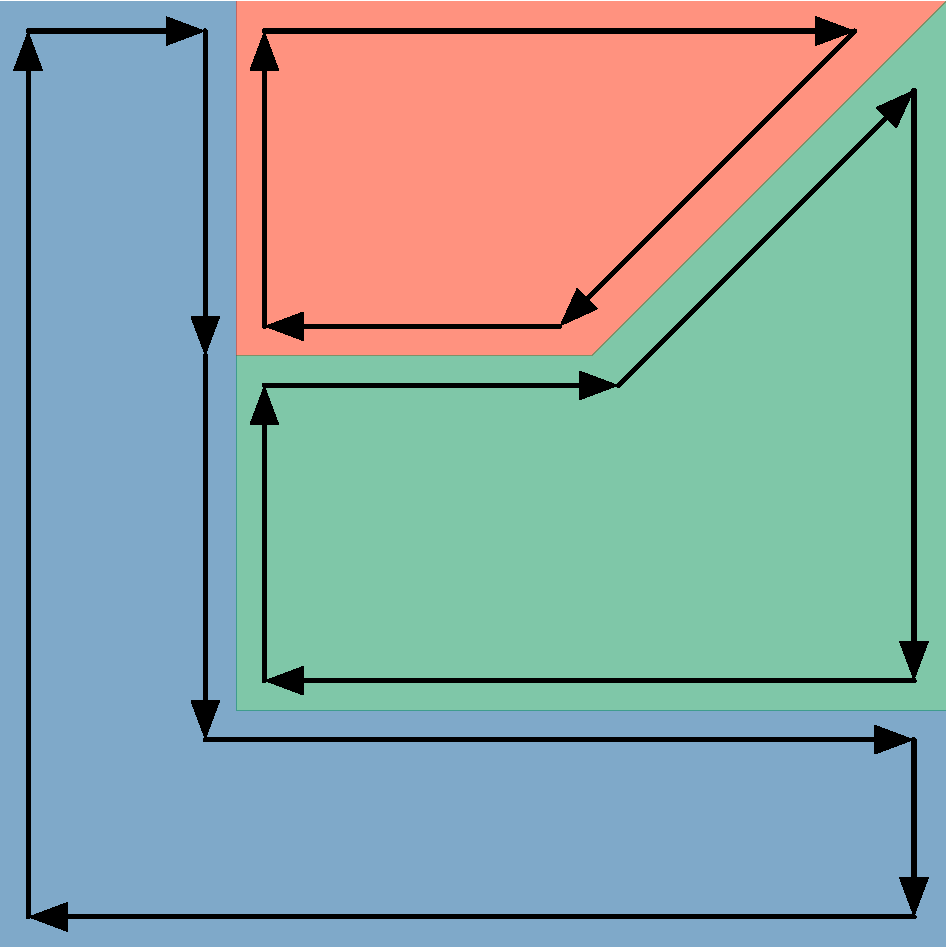
\includegraphics[width=\linewidth]{figs/cmaps-orientation-2}
\caption{}%
\label{subfig:cmaps-orientation-2}
\end{subfigure}\\
\caption{Every connected component in a combinatorial map has two possible orientations.
Here, the arrows are darts.
Note how a 2D combinatorial map is equivalent to a half-edge data structure.}%
\label{fig:cmaps-orientation}
\end{figure}

While the triangulation analogy is useful, visually representing darts as simplices is cumbersome and it does not work well in 3D.
For example, consider how the tetrahedra in Figure~\ref{subfig:cmap-3d} visually obstruct each other, which means that showing a more complex polyhedron than a cube is not ideal.
Because of this, most visualisations of generalised maps and combinatorial maps skip the vertices for 2-dimensional elements and higher, resulting in something that looks like a half-edge data structure (Figure~\ref{fig:2dcc}).

\begin{figure}
\centering
\begin{subfigure}{0.33\linewidth}
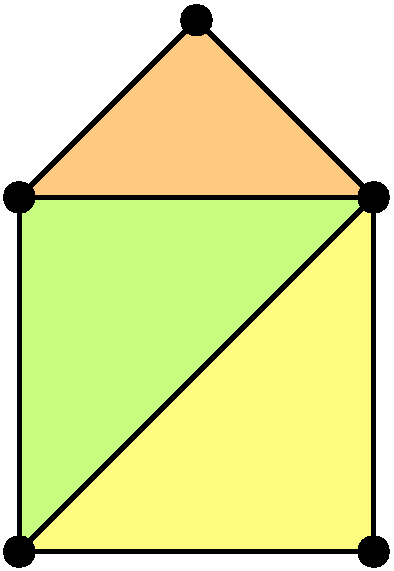
\includegraphics[scale=0.7]{figs/2dcc}
\caption{}%
\label{subfig:2dcc}
\end{subfigure}%
\quad
\begin{subfigure}{0.33\linewidth}
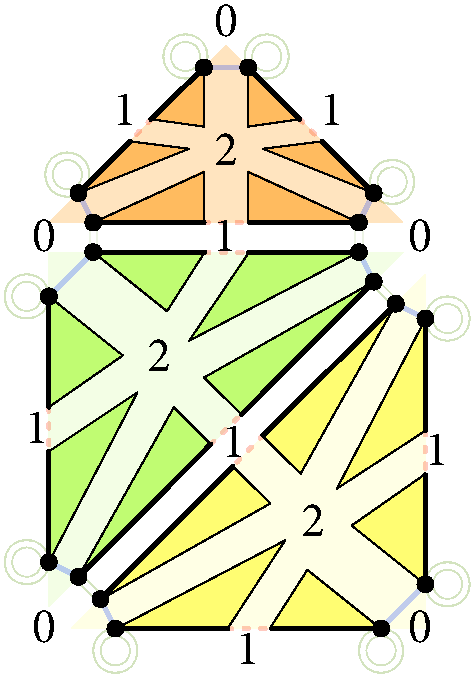
\includegraphics[scale=0.7]{figs/2dcc-gmap}
\caption{}%
\label{subfig:2dcc-gmap}
\end{subfigure}\\
\begin{subfigure}{0.33\linewidth}
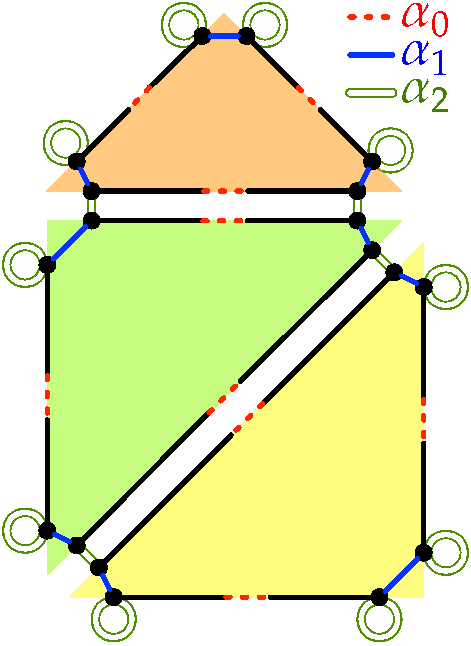
\includegraphics[scale=0.7]{figs/2dcc-alphas}
\caption{}%
\label{subfig:2dcc-alphas}
\end{subfigure}%
\quad
\quad
\begin{subfigure}{0.33\linewidth}
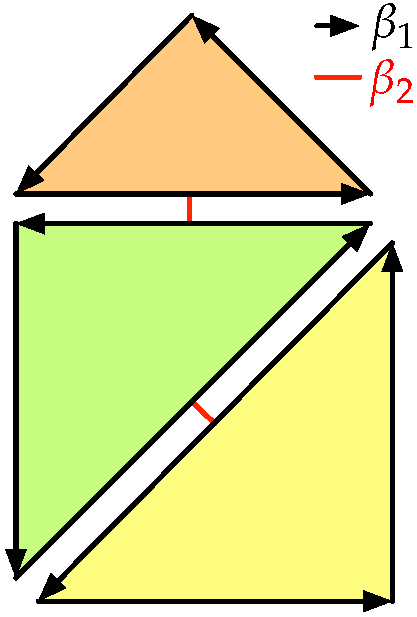
\includegraphics[scale=0.7]{figs/2dcc-betas}
\caption{}%
\label{subfig:2dcc-betas}
\end{subfigure}\\
\caption{(a) Three polygons, (b) their simplices while represented as a 2D generalised map, and alternative geometric interpretations of them as (c) a 2D generalised map and (d) a combinatorial map.}%
\label{fig:2dcc}
\end{figure}

Except for the special case of \(\beta_1\), it is important to note that applying the operation to switch from a dart to its neighbour twice results in returning to the same dart.
Since such an operation is equal to its own inverse, it is known mathematically as an \emph{involution}.
As for \(\beta_1\), it forms a loop of darts around a face that eventually returns to the original dart, and it is thus known instead as a \emph{permutation}.

\subsection{Orbits and sewing}

Starting from a given dart \(d\), the operation to obtain all the darts connected to it while following only the permutations/involutions corresponding to certain dimensions is known as an \emph{orbit} of \(d\).

Among these orbits, the most important one is the one to obtain all the darts belonging to a particular \emph{cell}, \ie\ a vertex, edge, face, or volume.
As we discussed previously, changing the \(i\)-dimensional cell (\(i\)-cell) of a dart, \ie\ applying \(\alpha_i\) or \(\beta_i\), means switching to an adjacent \(i\)-cell.
By the opposite logic, the orbit that obtains all the darts of an \(i\)-dimensional cell is the one that follows all the permutations and involutions except for \(\alpha_i\) or \(\beta_i\) (Figure~\ref{fig:darts-of-cell}).
For an \(n\)-dimensional generalised map, we can denote this as \(\langle \alpha_0, \ldots, \alpha_{i-1}, \alpha_{i+1}, \ldots, \alpha_n \rangle(d)\), and for an \(n\)-dimensional combinatorial map, we can denote this as \(\langle \beta_1, \ldots, \beta_{i-1}, \beta_{i+1}, \ldots, \beta_n \rangle(d)\).

\begin{figure}
\centering
\begin{subfigure}{0.4\linewidth}
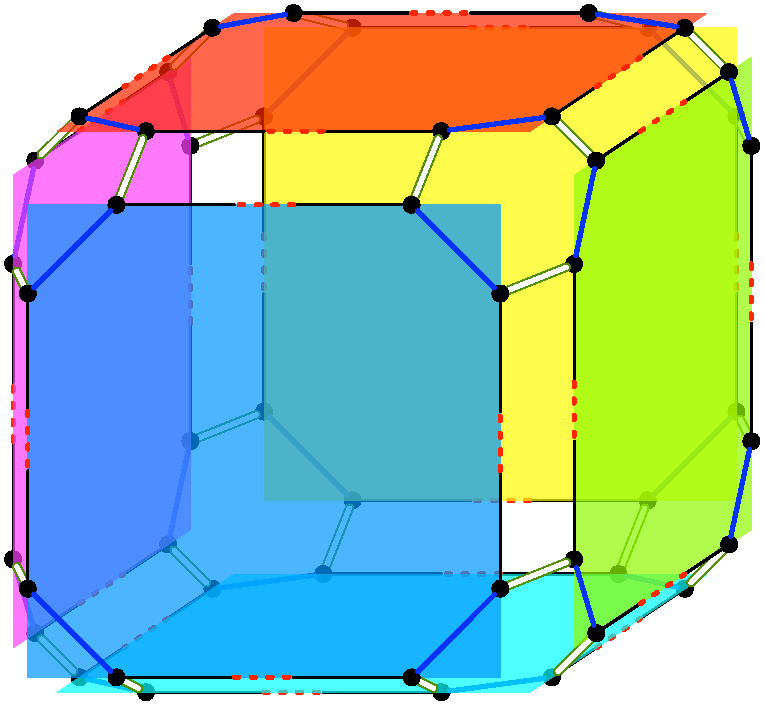
\includegraphics[width=\linewidth]{figs/darts-of-cell-1}
\caption{}%
\label{subfig:darts-of-cell-1}
\end{subfigure}%
\quad
\begin{subfigure}{0.4\linewidth}
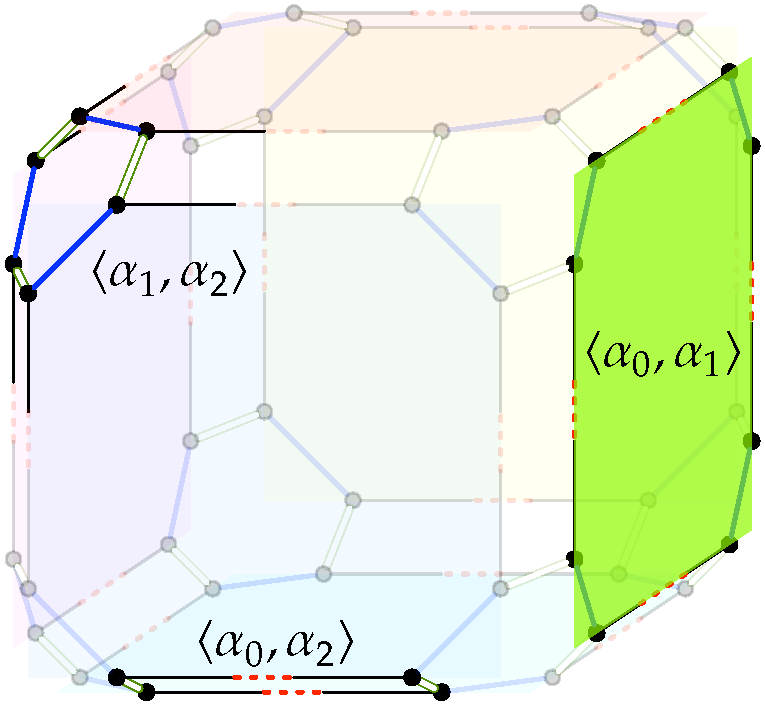
\includegraphics[width=\linewidth]{figs/darts-of-cell-2}
\caption{}%
\label{subfig:darts-of-cell-2}
\end{subfigure}\\
\caption{(a) A 3D generalised map of a cube, and (b) the orbits that represent one of its vertices, one of its edges and one of its faces.}%
\label{fig:darts-of-cell}
\end{figure}

Note that this means that the objects of any dimension are thus defined as \emph{sets of darts}.
While this is normal for faces and volumes in most other data structures, this applies also to vertices and edges in generalised and combinatorial maps.

Another important orbit is the one that obtains all the darts belonging to an \(i\)-cell within a \(j\)-cell, where \(i < j\).
This can be obtained using the orbit that follows all the permutations and involutions up to \(j-1\) except for \(\alpha_i\) or \(\beta_i\).
For instance, the darts belonging to an edge within a single volume (without obtaining the darts of the same edge but on other volumes) are obtained as \(\langle \alpha_0, \alpha_2 \rangle(d)\) in a generalised map and \(\langle \beta_2 \rangle(d)\) in a combinatorial map.

An important characteristic of orbits is that if they are implemented with some care, it is possible to use them to iterate over the darts of a cell in a consistent order.
This is the basis of the operation that is used to construct generalised and combinatorial maps, which is called \emph{sewing}.
In order to sew together two \(i\)-dimensional objects, the \(i\)-sewing operation starts from two corresponding darts on a common (\(i-1\))-cell but on different \(i\)-cells (Figure~\ref{fig:3-sew}).
It then proceeds to do a parallel traversal of each of their (\(i-1\))-orbits while connecting corresponding darts with \(\alpha_i\) (for a g-map) or \(\beta_i\) (for a c-map).

\begin{figure}
\centering
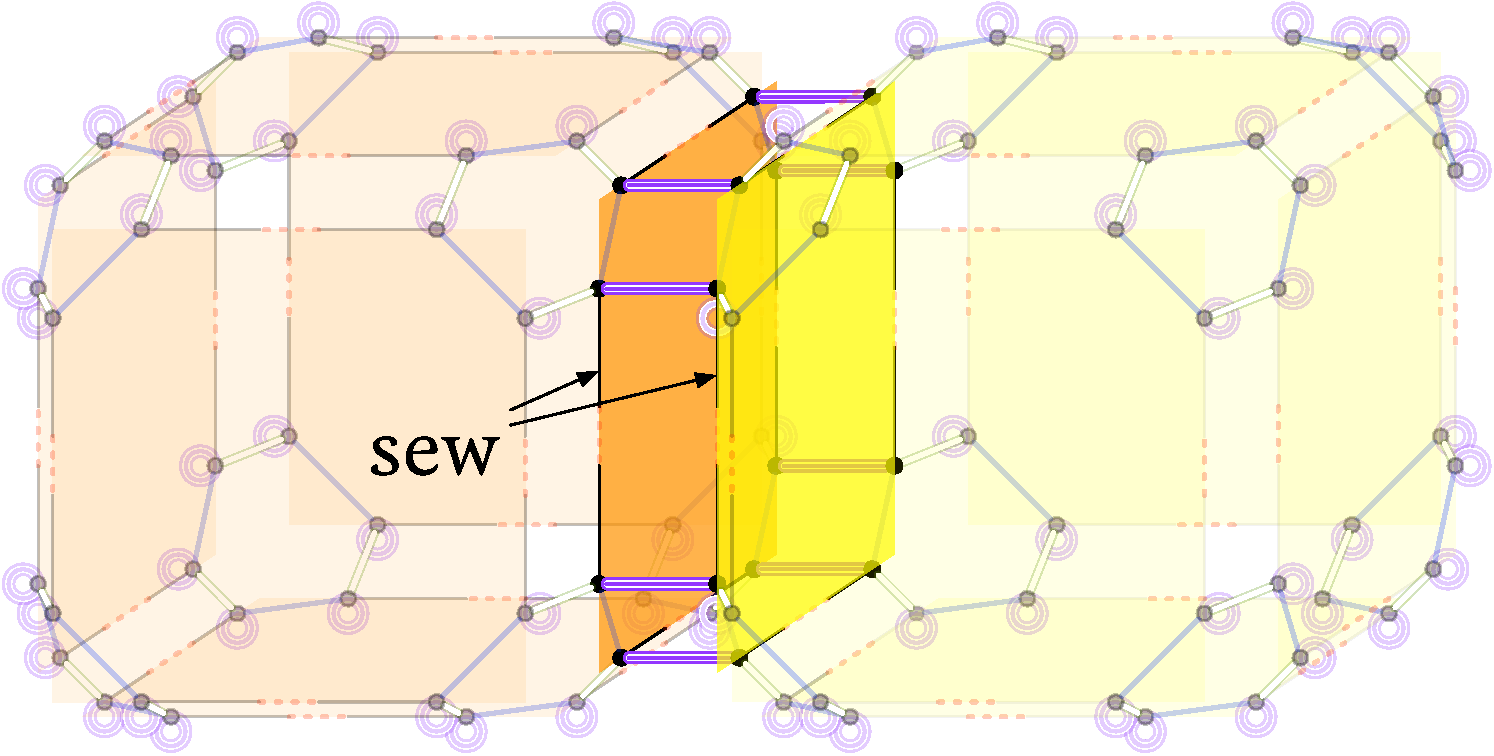
\includegraphics[width=0.8\linewidth]{figs/3-sew}
\caption{A 3-sewing operation to connect two cubes along a common face.
Note that the operation should start from corresponding darts on either volume.}%
\label{fig:3-sew}
\end{figure}

This process can be used to simply connect adjacent \(i\)-dimensional objects together, but it can also be used to create (\(i+1\))-dimensional objects.
For example, two vertices can be 0-sewn to create an edge (in a g-map), adjacent pairs of edges in a loop can be 1-sewn to create a face, a set of faces enclosing a volume can be 2-sewn along their common edges to create a volume.

\section{Implementing generalised and combinatorial maps}

With data structures for geometric modelling, it is often useful to separate them into two parts: (i) a combinatorial structure that describes the primitives and the relationships between them, and (ii) an embedding structure that maps the primitives to space and stores additional information (\eg\ attributes).
This division is particularly clear in generalised and combinatorial maps.

The most common way to implement a generalised or combinatorial map encodes each dart as a pair of tuples: one for the combinatorial part and one for its embedding.
The combinatorial tuple contains all the permutations and involutions of the dart in order according to their dimension.
For instance, these can be pointers or memory addresses of other darts, or something like ids (in which case the tuple should also contain an id for the dart).
When no objects are connected to a dart through that permutation/involution, a special marker can be used (\eg\ null or zero).

As for the embedding tuple, it generally consists of links to specific structures to store the geometry and attributes for the cell of each dimension that a dart belongs to.
For example, the first element of the tuple could then be a link to a 0-embedding structure, which then contains a list of attributes about the vertex of that dart, the next element could be a link to a 1-embedding structure with information about its edge, and so on.
If no embedding information is needed for the cells of a particular dimension, the corresponding item in the tuple can be omitted, although it is generally desirable to have at least a basic embedding structure with an id.

Regarding the geometric information, in the simplest case, where all geometries are linear (\ie\ line segments, polygons and polyhedra), the 0-embedding structure of a particular vertex can just contain its point coordinates.
From these points, we can linearly interpolate the higher-dimensional geometries by assuming that line segments connect two points and polygons are bounded by (roughly coplanar) line segments.
This kind of data structure with the linear geometries assumption is known as a \emph{linear cell complex}.

More complex geometries can be however stored in a generalised or combinatorial map using the higher-dimensional embeddings.
For instance, we can store the control points for a B\'ezier curve in its 1-embedding structure, or the ones for a B\'ezier surface in its 2-embedding structure.

%%%
%
\section{Exercises}

\begin{enumerate}
	\item Why do barycentric triangulations only work well with roughly convex polygons/polyhedra?
	\item Look at the differences between g-maps and c-maps. Can you tell why implementing algorithms on c-maps is often much harder than on g-maps?
	\item What are the equivalent operations between the DCEL and a 2D combinatorial map?
	\item Rather than storing links to special embedding structures for each dimension in the embedding tuple of a dart, it is also possible to store point coordinates directly. Why is this usually a bad idea?
\end{enumerate}



%%%
%
\section{Notes and comments}

\(n\)-dimensional generalised and combinatorial maps were developed by \citet{Lienhardt94} as a generalisation of 2D combinatorial maps~\citep{Edmonds60}.
Independently, the cell-tuple structure~\citep{Brisson89} was developed as a generalisation of the quad-edge \citep{Guibas85} data structure in 2D and the facet-edge data structure \citep{Dobkin87} in 3D.
The two data structures (generalised maps and the cell-tuple) are basically equivalent.
However, for a more in-depth look at combinatorial maps, see \citet{Damiand14} instead.

Chains of maps \citep{Elter94} supplement the approach used in generalised maps and combinatorial maps with an incidence graph, which can be used to support non-manifolds, but they are rarely used because of their extremely high space requirements.

Moka\footnote{\url{http://moka-modeller.sourceforge.net}} is a nice free modeller that uses generalised maps.
There are also good implementations of generalised maps\footnote{\url{https://doc.cgal.org/latest/Generalized_map/index.html}} and combinatorial maps\footnote{\url{https://doc.cgal.org/latest/Combinatorial_map/index.html}} in CGAL\@.
